% Unofficial University of Cambridge Poster Template
% https://github.com/andiac/gemini-cam
% a fork of https://github.com/anishathalye/gemini
% also refer to https://github.com/k4rtik/uchicago-poster

\documentclass[final]{beamer}

% ====================
% Packages
% ====================

\usepackage[T1]{fontenc}
\usepackage{lmodern}
\usepackage[orientation=portrait,size=a0,scale=1.12]{beamerposter}
\usetheme{gemini}
\usecolortheme{nott}
\usepackage{graphicx}
\usepackage{booktabs}
\usepackage{tikz}
\usepackage{pgfplots}
\pgfplotsset{compat=1.14}
\usepackage{anyfontsize}
\usepackage{multirow}
\usepackage{subcaption} 
\usepackage{xcolor}
\usepackage{fancybox}
\usepackage[most]{tcolorbox}

% ====================
% Lengths
% ====================

% If you have N columns, choose \sepwidth and \colwidth such that
% (N+1)*\sepwidth + N*\colwidth = \paperwidth
\newlength{\sepwidth}
\newlength{\colwidth}
\setlength{\sepwidth}{0.025\paperwidth}
\setlength{\colwidth}{0.45\paperwidth}

\definecolor{darkgreen}{rgb}{2, 48, 32}

\newcommand{\separatorcolumn}{\begin{column}{\sepwidth}\end{column}}

% ====================
% Title
% ====================

\title{From FusHa to Folk: Exploring Cross-Lingual Transfer in Arabic Language Models}

\author{Abdulmuizz Khalak \and Abderrahmane Issam \and Gerasimos Spanakis}

% \institute[shortlist]{ Maastricht University }

% ====================
% Footer (optional)
% ====================

% \footercontent{
%   \href{https://utfpr.edu.br/ct/ppgca}{utfpr.edu.br/ct/ppgca} \hfill
%   Mostra de Trabalhos do PPGCA --- TechTalks 2024 \hfill
%   \href{mailto:ppgca-ct@utfpr.edu.br}{ppgca-ct@utfpr.edu.br}}

\footercontent{
  \href{https://www.maastrichtuniversity.nl/nl}{\textbf{Maastricht University}} \hfill
  \textbf{VarDial 2026 Poster} \hfill
  \href{mailto:a.khalak@student.maastrichtuniversity.nl}{\textbf{a.khalak@student.maastrichtuniversity.nl}}}
% (can be left out to remove footer)


% ====================
% Logo (optional)
% ====================

% use this to include logos on the left and/or right side of the header:
% \logoright{
\includegraphics[height=4cm]{logos/VOXReality-logo.png}}
\logoleft{\hspace{3ex}
\includegraphics[height=3.5cm]{logos/maastricht_logo.svg.png}}

% ====================
% Body
% ====================

\begin{document}

\begin{frame}[t]
\begin{columns}[t]
\separatorcolumn

\begin{column}{\colwidth}

  \begin{block}{Introduction}
  \begin{tcolorbox}[
    colback=green!5!white,   % Background color (e.g., 5% blue tint)
    colframe=blue!75!black, % Frame color
    boxrule=0.pt,          % Frame thickness
    arc=4pt                 % Slight corner rounding
]
      \textbf{How to bridge between the input (speech) and the output (text) modalities in E2E-ST?}
    \begin{itemize}
    \item Finding an alignment between speech and text transcriptions.
    \item Training with an objective that maximizes the alignment.
  \end{itemize}
  \end{tcolorbox}
  
\begin{figure}[t]
    \centering
    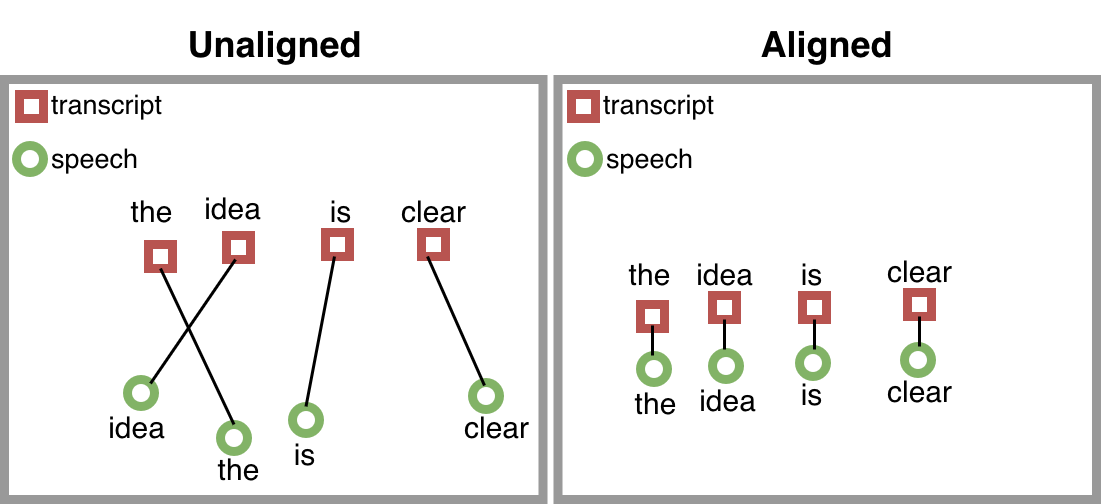
\includegraphics[width=0.84\textwidth]{figures/alignment.png}
\end{figure}

\begin{itemize}
    \item To find an alignment between speech and text, previous work require an alignment tool but \textbf{CMOT} does not.
    \item We propose \textbf{DTW-Align}, which relies on DTW to align speech and text representations during training. 
    \item Unlike CMOT, our method guarantees monotonic alignment and that all tokens are aligned.
    % Compared to state-of-the-art, our method guarantees monotonic alignment and that all tokens are aligned. 
\end{itemize}

  \begin{figure}[t]
    \centering
    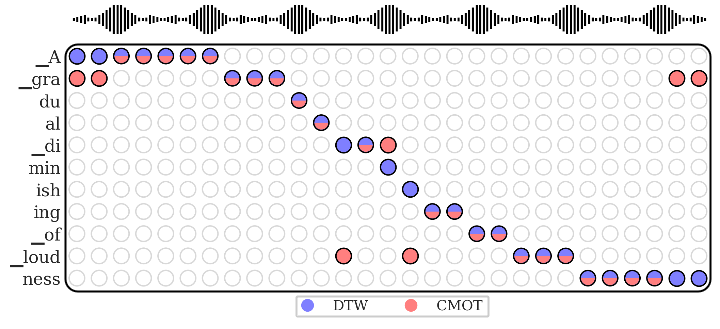
\includegraphics[width=0.84\textwidth]{figures/dtw_intro.png}
\end{figure}
  
  \end{block}
  
% \vspace{-0.3cm}
  \begin{block}{Methodology}
\begin{itemize}
    \item DTW-Align is used to align speech frames and text tokens.
    \item The alignment is used for \textbf{mixup training}.
\end{itemize}
    \begin{figure}[t]
        \centering
        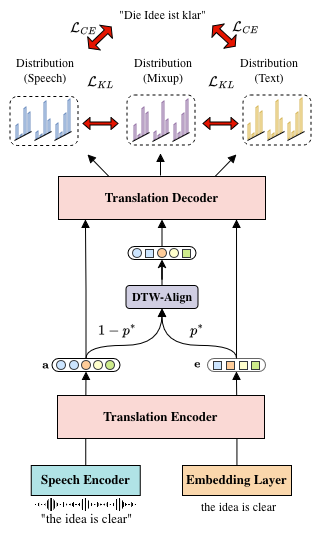
\includegraphics[width=0.45\textwidth]{figures/dtw_arch.png}
    \end{figure}
    
    % This is the first minipage (left)
    \begin{minipage}[t]{0.5\textwidth} % Minipage for the left figure
        \textbf{DTW-Align:}
        \centering
        \begin{figure}[H]
            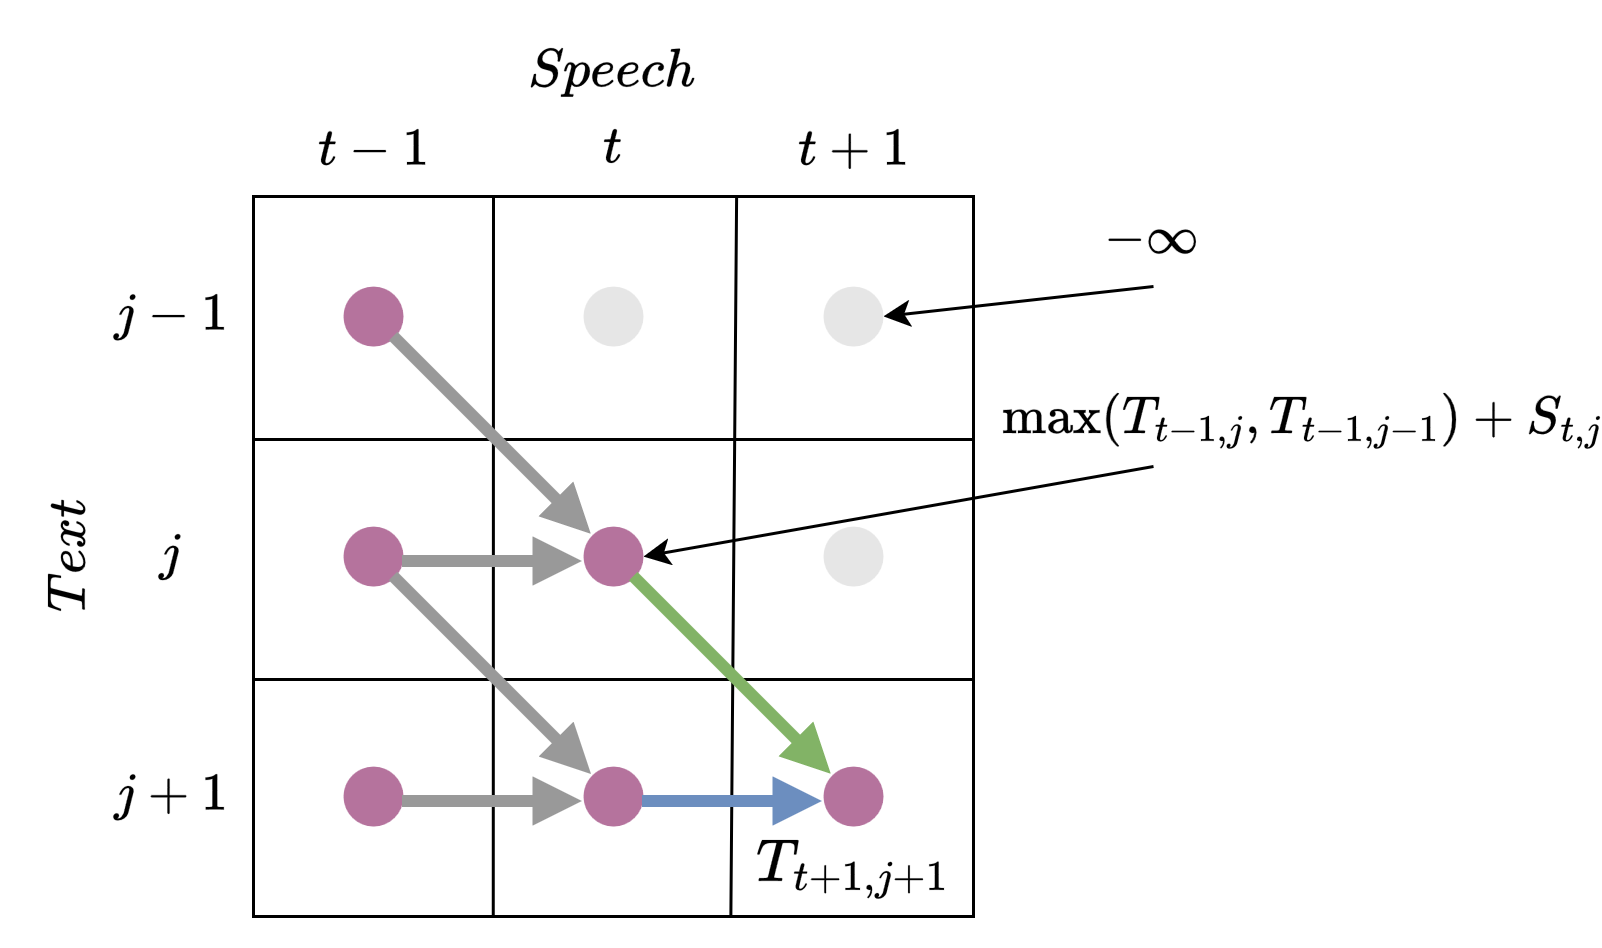
\includegraphics[width=\linewidth]{figures/dtw_method_poster_export.png}
        \end{figure}
    \end{minipage}
    \hfill
    \begin{minipage}[t]{0.5\textwidth} % Minipage for the right figure
        \textbf{Discrete vs. Interpolation Mixup:}
        \vspace{2cm}
        \centering
        \begin{figure}[H]
            
\includegraphics[width=\linewidth]{figures/mixup_export.png}
        \end{figure}
    \end{minipage}

  \end{block}

\end{column}

\separatorcolumn

\begin{column}{\colwidth}

\begin{block}{Main Results}
\begin{itemize}
    \item CMOT, DTW-Align, and DTW-Align-Discrete achieve the best results against other baselines.
\end{itemize}
\begin{table}
    \centering
    \label{tab:model-comparison}
    \begin{tabular}{lccccccc}
    \toprule
        \textbf{Model} & \textbf{En-De} & \textbf{En-Ca} & \textbf{En-Ar} & \textbf{De-En}  & \textbf{Fr-En} & \textbf{Es-En} & \textbf{Avg.} \\
    \midrule
        % Model & En-De & En-Ca & En-Ar & De-En & Fr-En & Es-En & Avg. \\ \hline
        Revist-ST \dag & 17.5 & 22.9 & 12.3 & 14.1 & 26.9 & 15.7 & - \\
        U2TT (Large) \dag & - & - & - & 16.7 & 27.4 & 28.1 & - \\ 
        DUB (Large) \dag & - & - & - & 19.5 & 29.5 & \textbf{30.9} & - \\
        SRPSE \dag & - & - & - & 21.4 & 29.3 & - & - \\
        CoVoST-2 \dag & 18.4 & 23.6 & 13.9 & 18.9 & 27.0 & 28.0 & 21.6 \\
        CTC+OT \dag & 20.6 & 26.5 & 15.3 & 20.4 & 28.4 & 29.2 & 23.4 \\
        HuBERT-Transformer & 21.4 & 27.4 & 15.7 & 21.8 & 28.4 & 28.0 & 23.8 \\ 
        CMOT & \textbf{21.8} & 28.2 & \textbf{16.2} & 23.6 & 30.9 & 29.6 & \textbf{25.0} \\ 
        NFA-Align & 21.4 & 28.1 & 16.0 & 23.5 & 30.9 & 29.8 & 24.9 \\ 
        \fcolorbox{green}{white}{DTW-Align-Discrete} & 21.7 & \textbf{28.3} & \textbf{16.2} & 23.5 & \textbf{31.0} & 29.4 & \textbf{25.0} \\ 
        \fcolorbox{green}{white}{DTW-Align} & \textbf{21.8} & 28.2 & 16.1 & \textbf{23.7} & 30.8 & 29.5 & \textbf{25.0} \\ 
    \bottomrule
    \end{tabular}
    \label{table:main_results}
    \caption*{\dag indicates that the results are as reported in the original work.}
\end{table}
% \begin{figure}[ht]
%     % \setlength{\fboxsep}{1pt} 
%     \centering
%     \begin{subfigure}{0.48\textwidth}
%         \centering
%         \begin{tcolorbox}[colframe=red, colback=white, boxsep=0pt]
%         \includegraphics[width=\textwidth]{figures/probing_poster.png}
%         \end{tcolorbox}
%     \end{subfigure}
%     \hfill
%     \begin{subfigure}{0.48\textwidth}
%         \centering
%         \begin{tcolorbox}[colframe=green, colback=white, boxsep=0pt]
%         \includegraphics[width=\textwidth]{figures/similarity_poster.png}
%         \end{tcolorbox}
%     \end{subfigure}
% \end{figure}
  \end{block}

\begin{block}{Alignment Accuracy and Training time}
\begin{itemize}
    \item DTW-Align is significantly faster and more accurate than CMOT.
\end{itemize}
    \begin{table}
    \centering
    \begin{tabular}{llcccc}
        \toprule
        & \textbf{Method} & \textbf{Accuracy} $\uparrow$ & \textbf{Execution Time} $\downarrow$ & \textbf{Train Time} $\downarrow$ \\
        \midrule
        & CMOT & 26\% & 97.89 & 14:20:53 \\
        & \fcolorbox{green}{white}{DTW-Align} & \textbf{45\%} & \textbf{2.91} & \textbf{6:48:14} \\
        \bottomrule
    \end{tabular}
    \label{table:acc_time}
    \end{table}
\end{block}

\begin{block}{Synthetic Low Resource Setting}
\begin{itemize}
    \item DTW-Align achieves better results in low resource settings.
    \item Indicates that alignment accuracy is more important in low resource scenarios.
    \item Shows that interpolation mixup is more robust and data efficient.
\end{itemize}
    \begin{table}[ht]
    \centering
    \label{tab:model-comparison}
    % \small
    \begin{tabular}{lccccccc}
    \toprule
        \textbf{Model} & \textbf{En-De} & \textbf{En-Ca} & \textbf{En-Ar} & \textbf{De-En}  & \textbf{Fr-En} & \textbf{Es-En} & \textbf{Avg.} \\
    \midrule
        HuBERT-Transformer & 6.4 & 8.7 & 2.2 & 1.8 & 3.2 & 2.9 & 4.2 \\ 
        CMOT & 6.6 & 9.6 & 2.7 & 2.8 & 8.5 & 7.5 & 6.3 \\ 
        \fcolorbox{green}{white}{DTW-Align-Discrete} & 6.8** & 9.6 & 2.8 & 2.7 & \textbf{8.6} & 7.9** & 6.4 \\ 
        \fcolorbox{green}{white}{DTW-Align} & \textbf{7.0**} & \textbf{9.8**} & \textbf{3.1**} & \textbf{2.9*} & \textbf{8.6} & \textbf{8.0**} & \textbf{6.6} \\ 
    \bottomrule
    \end{tabular}
    \end{table}
\end{block}

\begin{block}{Effect of the Mixup Probability}
\begin{itemize}
    \item Increasing the mixup probability $p^*$ (more text) hurts CMOT more.
    \item This is an implication of lower alignment accuracy.
\end{itemize}
    \begin{figure}
    \centering
    \begin{subfigure}{0.47\textwidth}
        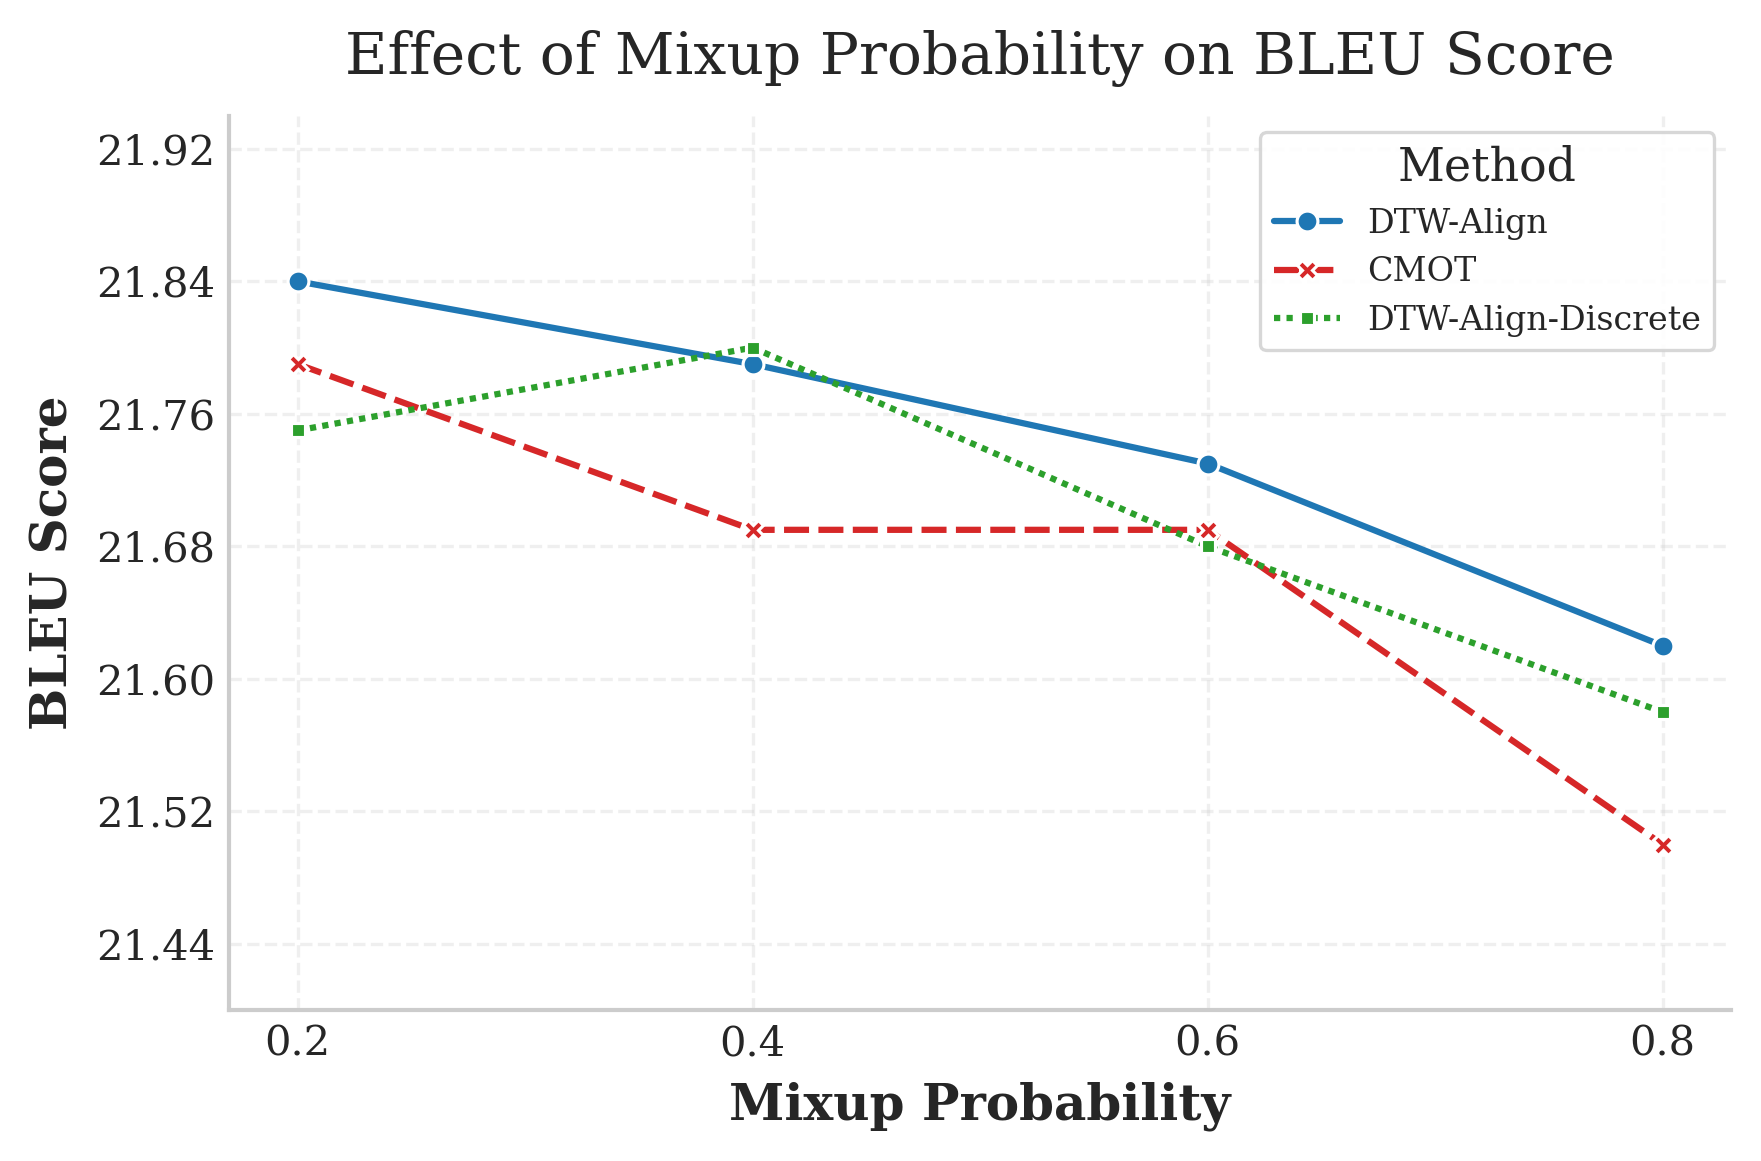
\includegraphics[width=1.0\textwidth]{figures/mixup_prob.png}
    \caption{En-De}
    \label{fig:high}
    \end{subfigure}
    \begin{subfigure}{0.47\textwidth}
        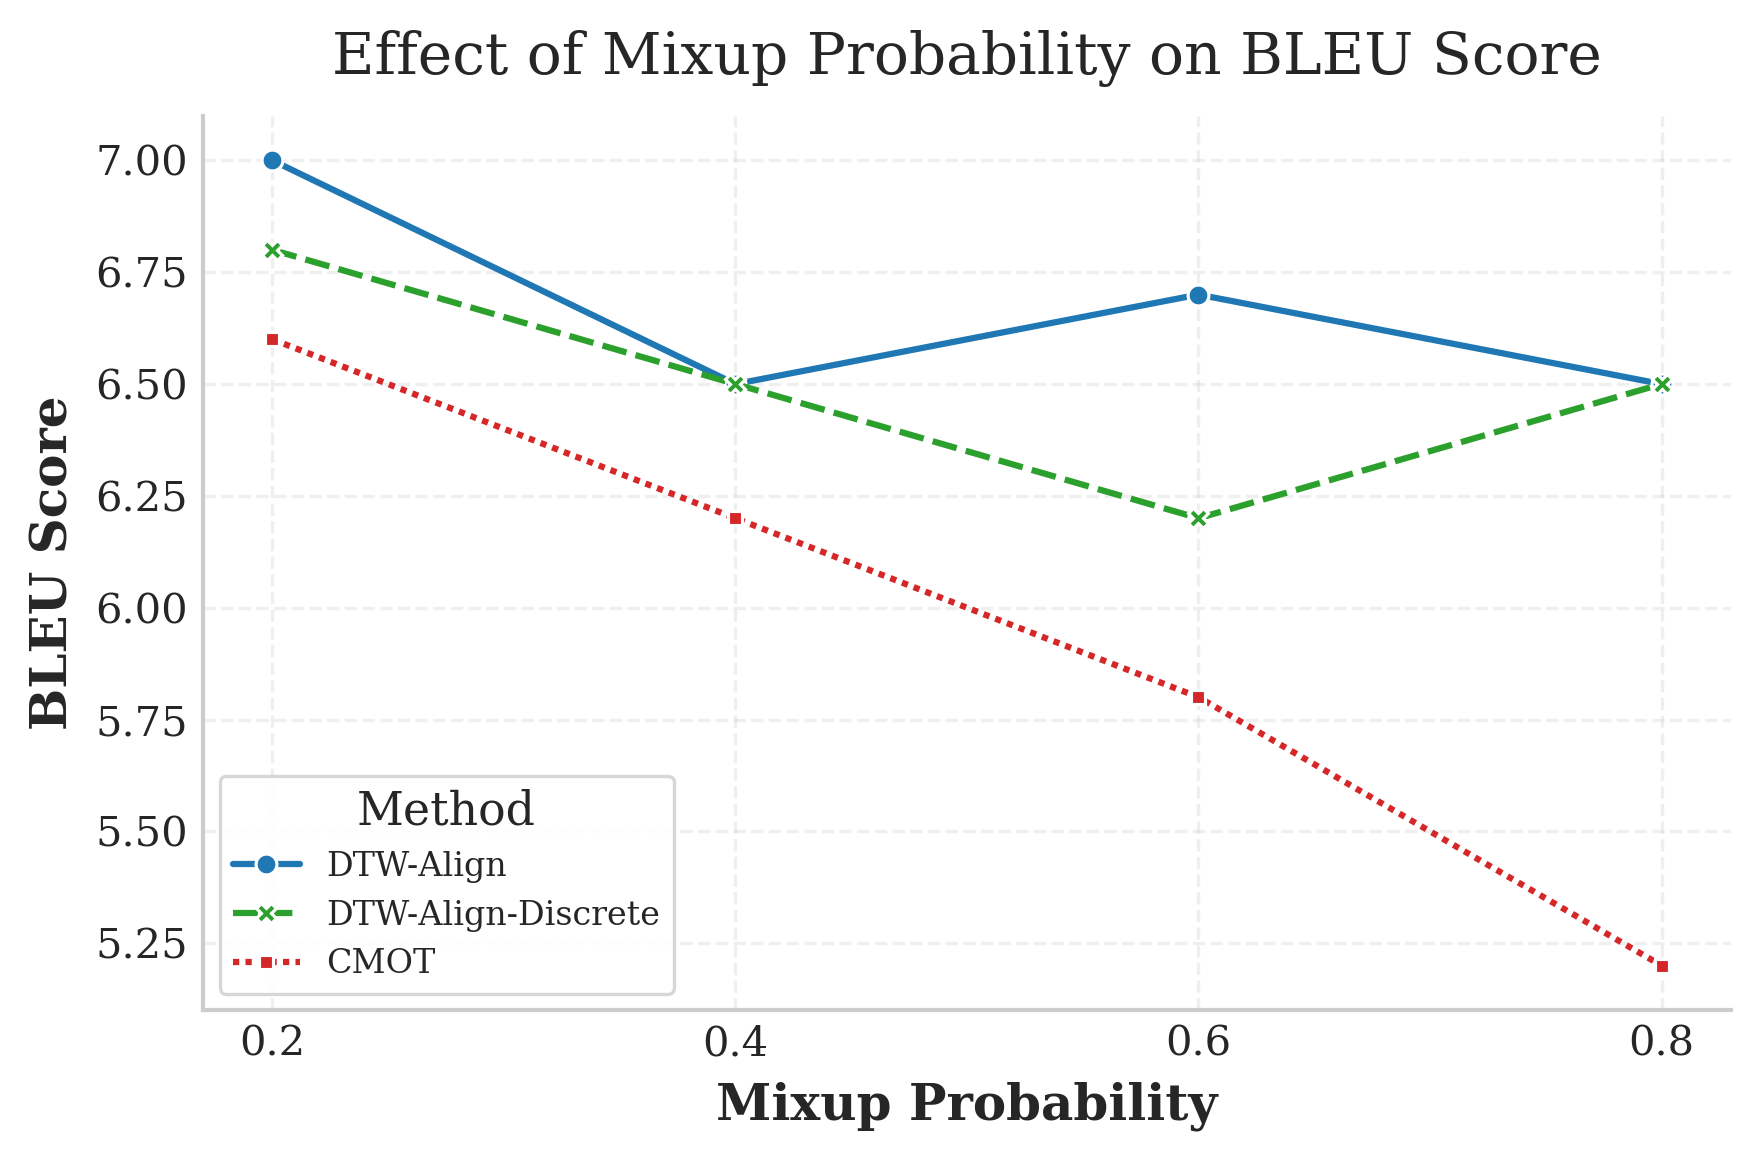
\includegraphics[width=1.0\textwidth]{figures/mixup_prob_lrs.png}
    \caption{En-De Low Resource}
    \label{fig:low}
    \end{subfigure}
\end{figure}
\end{block}

\begin{exampleblock}{Conclusion}
\large
    \begin{enumerate}
        \item We introduce DTW-Align, a method that \textbf{combines} DTW for alignment and interpolation mixup.
        \item DTW-Align achieves \textbf{similar results to CMOT} on 6 language directions.
        \item DTW-Align is \textbf{faster and more accurate} than CMOT for alignment.
        \item In a \textbf{low resource setting}, DTW-Align achieves \textbf{better results} than CMOT on all language directions.
    \end{enumerate}
    
\end{exampleblock}

\begin{figure}[h]
    \centering
    \begin{tcolorbox}[
        enhanced,
        colback=blue!5!white, % Light blue background
        colframe=blue!40!black, % Slightly darker blue frame
        title=\textbf{Get the Full Paper :)},
        fonttitle=\bfseries\large,
        boxsep=5pt,
        arc=5pt, % Rounded corners
        width=0.4\textwidth, % Control the total width of the box
        center title
    ]
        \centering
        
\includegraphics[width=0.4\linewidth]{logos/qr-code.png} % Use \linewidth here as it's inside the tcolorbox
        \vspace{0.5em}
        % {\small \itshape Scan to view the PDF.}
    \end{tcolorbox}
\end{figure}
\end{column}
\separatorcolumn


\end{columns}
\end{frame}

\end{document}
